\addcontentsline{toc}{chapter}{IntelliJ IDEA}
\chapter*{IntelliJ IDEA}
\stepcounter{chapter}
IntelliJ IDEA es un Entorno de desarrollo Integrado (EDI) o Integrated Development Environment (IDE) para lenguajes JVM\footnote{Java
    Kotlin
    Scala
    Groovy
    Clojure
    Fantom
    Ceylon
    Jython
    JRuby
    Frege
    Xtend
    Golo
    Concurnaas
    Yeti } 
%https://www.spec-india.com/blog/jvm-languages
diseñado para maximizar la productividad del desarrollador. Hace la tareas rutinarias y repetitivas proporcionando un completado inteligente de código, análisis de código estático, refactoriza, y permite enfocarse en el lado brillante del desarrollo de software.

IntelliJ IDEA es multiplataforma, que provee una experiencia consistente en Windows, madOS, y Linux. 
Soportea múltiples lenguajes, herramientas, frameworks, y tecnologías. 

IntelliJ IDEA viene en tres ediciones:
\begin{itemize}
\item \textbf{IntelliJ IDE Ultimate}: Es la edición comercial para JVM, web, y desarrollo corporativo. Incluye todas las características de la edición Community, soporta una variedad de frameworks al lado des servidor así como del front-end, servidor de aplicaciones, integración con base de datos y soporte de herramientas y mucho mas. 
\item \textbf{IntelliJ IDEA Community Edition:} Es la edición gratuita basado en Open-source para JVM y desarrollo Android.
\item \textbf{IntelliJ IDEA Edu:} Es la edición libre con lecciones incorporadas para aprender Java, Kotlin, y Scala. Tiene características especiales para profesores para crear su propio curso y gestionar el proceso de aprendizaje. 
\end{itemize}

La interfaz de usuario sigue el contexto y trae herramientas necesarias de forma automática para ayudar a minimizar el riesgo de interrumpir el flujo del desarrollador. 

Lo mejor de IntelliJ IDEA es su configurabilidad, es decir se puede configurar cualquier cosa. Por ejemplo el color del fuente, salida de la consola, depurador, resultados de búsqueda, etc. 

Tiene atajos de teclado para toda acción,casi, incluyendo la selección y intercambiar el editor y varias herramientas de windows. 

Uno de los más útiles accesos por teclado es el doble shift que abre el dialogo \textbf{Buscar en todo}, buscará entre todos los archivos, clases, y símbolos que pertenecen al proyecto e incluso entre las acciones del IDE. 
\begin{figure}[h]
\centering
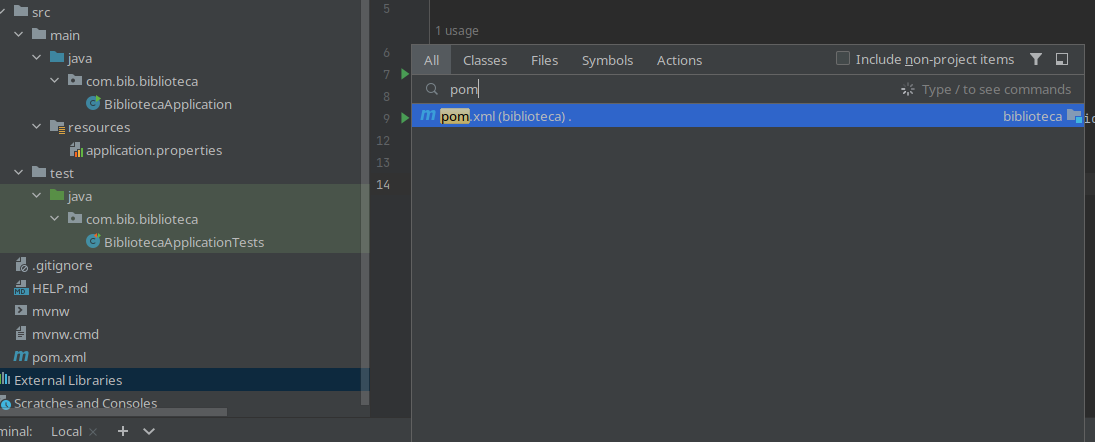
\includegraphics[width=10cm]{images/idea3}
\caption{Ventana de dialogo de buscar en todo}
\end{figure}
Puedes usar también esta acción para abrir cualquier herramienta de ventana. 

\section{Asistente al codificar}
El completado de código ayuda en la velocidad el proceso de codificar. El completado básico ayuda a completar los nombres de las clases, métodos, campos, y palabras reservadas.

El \textbf{completado inteligente} sugiere el más relevante símbolo aplicable en el contexto actual, cuando IntelliJ IDEA puede determinar el tipo apropiado. 
\section{Refactorización}
IntelliJ IDEA ofrece un comprensible conjunto de refactorización de código que permite una productividad significativa. Por ejemplo cuando renombra una clase, el IDE ayuda a actualizar todas las referencias a esa clase, sin siquiera seleccionar y solo requiere confirmación. 
\section{Terminal}
IntelliJ IDEA viene con terminal incorporado para trabajar con comandos de shell desde el IDE. Por ejemplo permite ejecutar comandos de Git. Soporta cmd.exe, bash, sh, etc. 
\section{Herramientas de construcción}
IntelliJ IDEA viene con un completo y funcional Gradle y Maven integrado que permite automatizar el proceso de construcción, empaquetado, correr pruebas, despliegue, y otras actividades. IntelliJ IDEA detecta y descarga automaticamente todo los repositorios requeridos y plugins, y no requiere usted configurar nada. 
\section{Control de Versiones}
IntelliJ IDEA está integrado con herramientas de control de versiones como, Git, Mercurial, Perforce, y Subversion. 
\section{Requerimientos del sistema e instalación}
Se puede ir a la siguiente dirección \url{https://www.jetbrains.com/idea/download/#section=linux}
\begin{figure}[h]
\centering
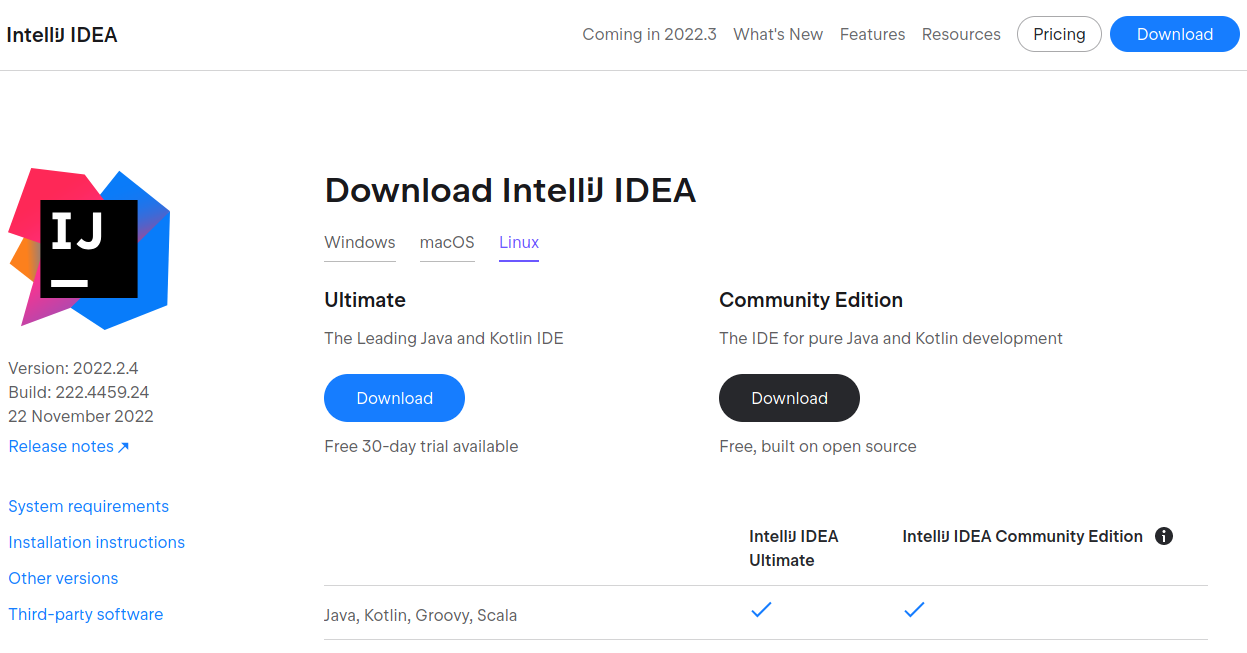
\includegraphics[width=10cm]{images/idea1}
\caption{Sección de descarga para Linux}
\end{figure}
En Linux cualquier distribución que soporte Gnome, KDE, o Unity DE puede soportarlo.
También se puede instalar por linea de comando:
\begin{verbatim}
sudo snap install intellij-idea-community --classic
or
sudo snap install intellij-idea-ultimate --classic

or
sudo snap install intellij-idea-educational --classic
\end{verbatim}
En el caso para el proyecto fue solo necesario descargar el comprimido en .tar, descomprimir y ejecutarlo por un comando el archivo idea.sh en la carpeta done se descomprimió:
\begin{figure}[h]
\centering
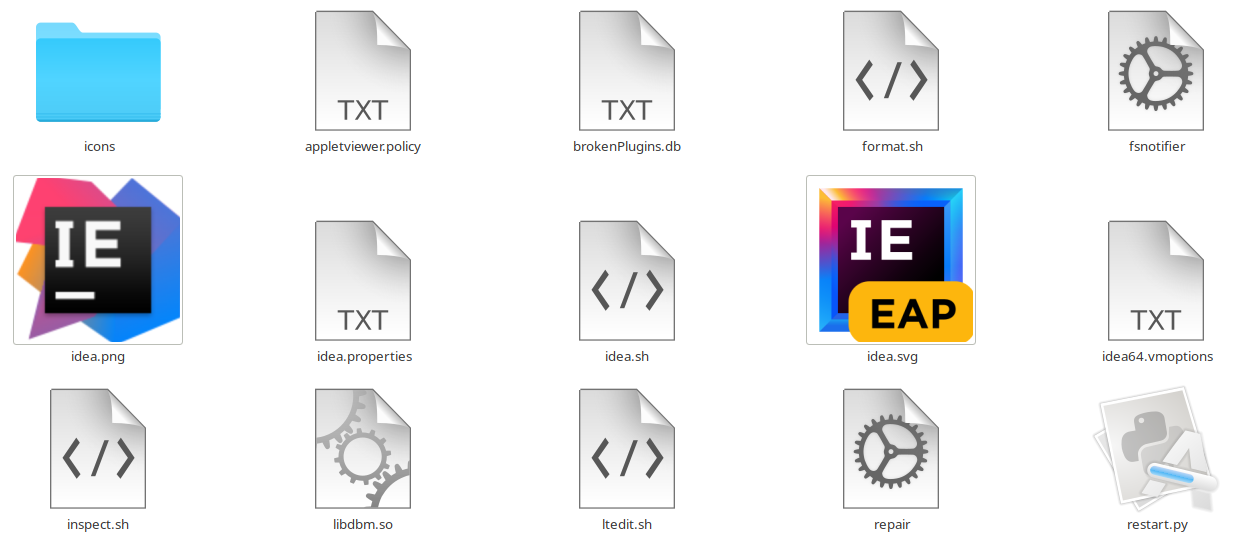
\includegraphics[width=10cm]{images/idea4}
\caption{Carpeta bin de la carpeta descomprimida}
\end{figure}

Una vez descomprimido el inicializado de Spring Boot y abierto en el editor IntelliJ IDEA no muestra lo siguiente:
\begin{figure}[h]
\centering
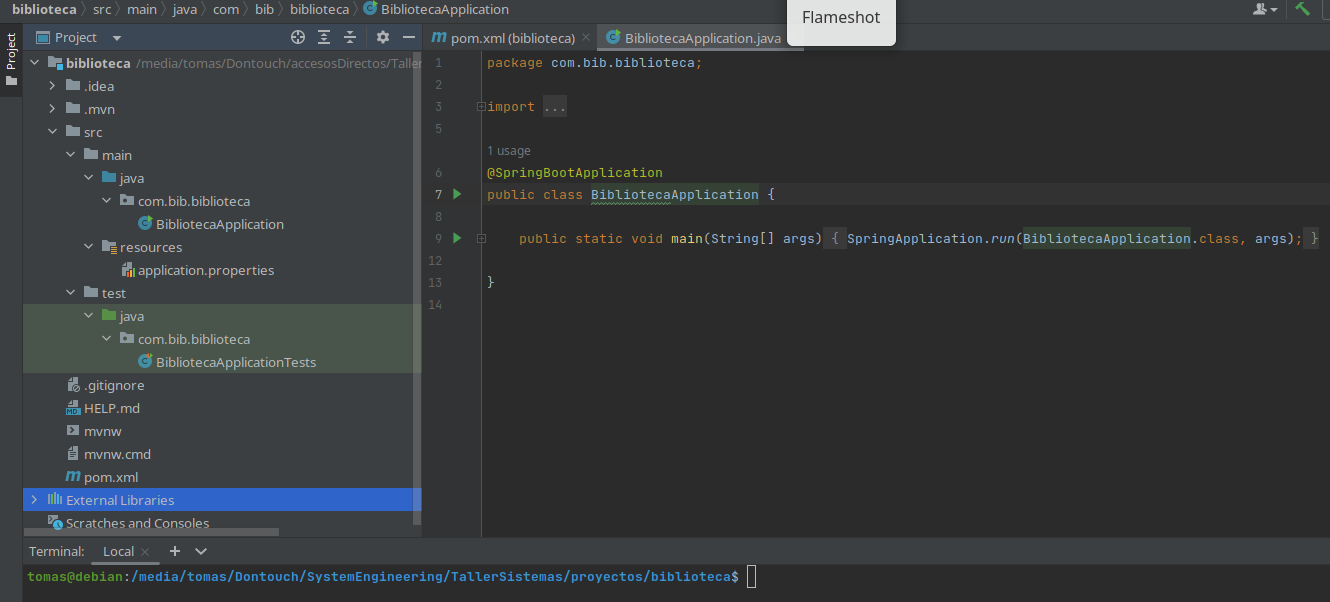
\includegraphics[width=10cm]{images/idea2}
\caption{El proyecto abierto por primera vez}
\end{figure}
